\documentclass[border=10pt]{standalone}

\usepackage{tikz}
\usepackage{tikzsymbols}
\usetikzlibrary{calc,patterns,shapes.geometric}

\def\centerarc[#1](#2)(#3:#4:#5){\draw[#1] ($(#2)+({#5*cos(#3)},{#5*sin(#3)})$) arc (#3:#4:#5);}

\begin{document}
	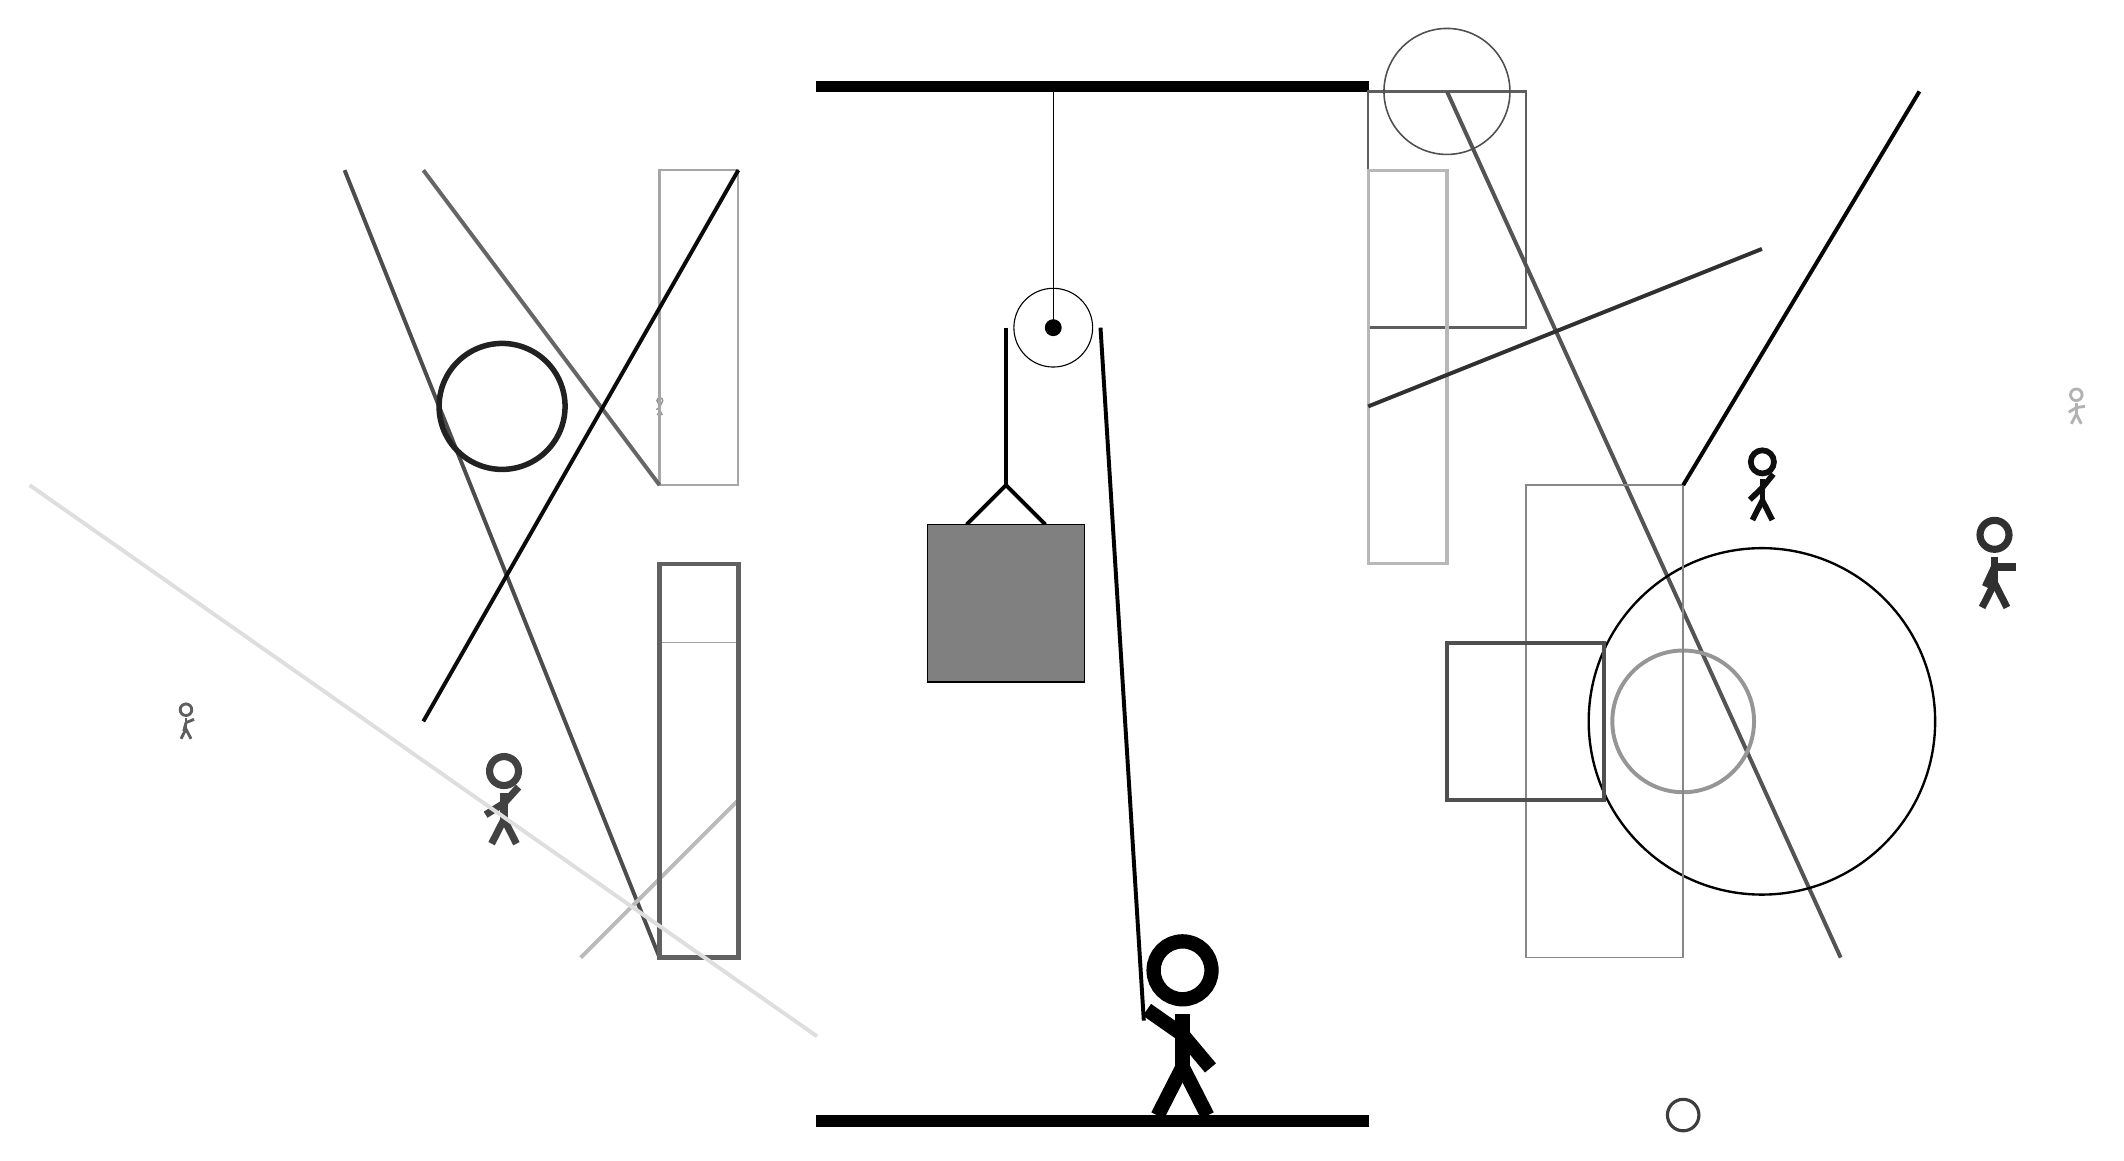
\begin{tikzpicture}
		%%%%% START %%%%%
		
		\draw[fill=black] (-2, 10) rectangle (5, 10.125);
		
		\draw (1, 7) circle (0.5);
		\draw[fill=black] (1, 7) circle (0.1);
		\draw (1, 10) -- (1, 7);
		
		\node[line width=0.6mm, color=black!42] at (-4, 6) {\Strichmaxerl[1][37][67]};
		
		\node[line width=0.3mm, color=black!74] at (-6, 1) {\Strichmaxerl[5][32][48]};
		\draw[line width=0.5mm, color=black!70](-4, -1) -- (-8, 9);
		\draw[line width=0.3mm, color=black!35] (-4, 5) rectangle (-3, 9);
		\draw [line width=0.7mm, color=black!87](-6, 6) circle (0.8);
		
		\draw[line width=0.3mm, color=black!63] (7, 7) rectangle (5, 10);
		
		\node[line width=0.3mm, color=black!94] at (10, 5) {\Strichmaxerl[4][44][51]};
		\draw[line width=0.5mm, color=black!67](6, 10) -- (11, -1);
		\node[line width=0.2mm, color=black!30] at (14, 6) {\Strichmaxerl[2][31][9]};
		\draw [line width=0.2mm, color=black!69](6, 10) circle (0.8);
		\draw[line width=0.4mm, color=black!28] (6, 4) rectangle (5, 9);
		\draw[line width=0.5mm, color=black!27](-5, -1) -- (-3, 1);
		\draw[line width=0.2mm, color=black!36] (-4, 3) rectangle (-3, -1);
		\draw[line width=0.5mm, color=black!81](5, 6) -- (10, 8);
		\draw [line width=0.3mm, color=black!100](10, 2) circle (2.2);
		\draw [line width=0.5mm, color=black!41](9, 2) circle (0.9);
		\draw[line width=0.6mm, color=black!62] (-3, -1) rectangle (-4, 4);
		\draw[line width=0.5mm, color=black!60](-7, 9) -- (-4, 5);
		\node[line width=0.5mm, color=black!81] at (13, 4) {\Strichmaxerl[5][65][0]};
		\draw[line width=0.2mm, color=black!47] (7, -1) rectangle (9, 5);
		\draw [line width=0.4mm, color=black!76](9, -3) circle (0.2);
		\draw[line width=0.5mm, color=black!98](9, 5) -- (12, 10);
		
		\draw[line width=0.5mm, color=black!69] (6, 3) rectangle (8, 1);
		\draw[line width=0.5mm, color=black!96](-3, 9) -- (-7, 2);
		\node[line width=0.4mm, color=black!63] at (-10, 2) {\Strichmaxerl[2][75][22]};
		
		\draw[line width=0.5mm, color=black!13](-2, -2) -- (-12, 5);
		
		\draw[line width=0.5mm] (-0.1, 4.5) -- (0.4, 5.0) -- (0.9, 4.5);
		\draw[fill=black!50] (-0.6, 4.5) rectangle (1.4, 2.5);
		
		\draw[line width=0.5mm] (0.4, 7) -- (0.4, 5.0);
		\centerarc[line width=0.5mm](1, 7)(0:180:0.6);
		\draw[line width=0.5mm](1.6, 7) -- (2.15, -1.8);
		
		\node at (2.6, -1.9) {\Strichmaxerl[10][-35][-50]};
		
		\draw[fill=black] (-2, -3) rectangle (5, -3.15);
		
		%%%%% END %%%%%
	\end{tikzpicture}
\end{document}